\documentclass{article}

\PassOptionsToPackage{numbers, compress}{natbib}
\usepackage[preprint]{neurips_2025}

\usepackage[utf8]{inputenc}
\usepackage[T1]{fontenc}
\usepackage{hyperref}
\usepackage{url}
\usepackage{booktabs}
\usepackage{amsfonts}
\usepackage{amsmath}
\usepackage{amssymb}
\usepackage{nicefrac}
\usepackage{microtype}
\usepackage{xcolor}
\usepackage{graphicx}
\usepackage{subcaption}
\usepackage{tikz}
\usetikzlibrary{positioning, arrows.meta, fit, backgrounds, calc}
\usepackage{algorithm}
\usepackage{algpseudocode}
\usepackage{enumitem}
\usepackage{wrapfig}
\usepackage{float}

\definecolor{cblue}{HTML}{2a78d6}
\definecolor{corange}{HTML}{eb6834}
\definecolor{caqua}{HTML}{1baf7a}
\definecolor{cmagenta}{HTML}{e87ba4}
\definecolor{cviolet}{HTML}{4a3aa7}
\definecolor{cyellow}{HTML}{eda100}
\definecolor{cink}{HTML}{52514e}
\definecolor{cgrid}{HTML}{e4e3df}

\hypersetup{colorlinks=true, linkcolor=cblue, citecolor=cblue, urlcolor=cblue}

% generated by make_figures.py -- do not edit
\newcommand{\BasePong}{+17.1}
\newcommand{\BasePongStd}{1.6}
\newcommand{\BaseLazy}{-10.1}
\newcommand{\BaseLazyStd}{1.2}
\newcommand{\BaseFrozen}{-13.4}
\newcommand{\BaseFrozenStd}{2.0}
\newcommand{\BaseSeeds}{3}
\newcommand{\BaseWon}{0}
\newcommand{\BaseLazyMin}{-11.3}
\newcommand{\BaseLazyMax}{-8.4}
\newcommand{\BaseWorstGame}{-17}
\newcommand{\DynPong}{+17.8}
\newcommand{\DynPongStd}{0.0}
\newcommand{\DynLazy}{+0.2}
\newcommand{\DynLazyStd}{0.0}
\newcommand{\DynFrozen}{+11.3}
\newcommand{\DynFrozenStd}{0.0}
\newcommand{\DynSeeds}{1}
\newcommand{\DynWon}{53}
\newcommand{\DynLazyMin}{+0.2}
\newcommand{\DynLazyMax}{+0.2}
\newcommand{\DynWorstGame}{-9}
\newcommand{\GatedPong}{+19.4}
\newcommand{\GatedPongStd}{0.0}
\newcommand{\GatedLazy}{-4.9}
\newcommand{\GatedLazyStd}{0.0}
\newcommand{\GatedFrozen}{-1.3}
\newcommand{\GatedFrozenStd}{0.0}
\newcommand{\GatedSeeds}{1}
\newcommand{\GatedWon}{6}
\newcommand{\GatedLazyMin}{-4.9}
\newcommand{\GatedLazyMax}{-4.9}
\newcommand{\GatedWorstGame}{-10}
\newcommand{\OursSixtyPong}{+17.5}
\newcommand{\OursSixtyPongStd}{0.4}
\newcommand{\OursSixtyLazy}{+9.4}
\newcommand{\OursSixtyLazyStd}{6.3}
\newcommand{\OursSixtyFrozen}{+17.9}
\newcommand{\OursSixtyFrozenStd}{0.6}
\newcommand{\OursSixtySeeds}{2}
\newcommand{\OursSixtyWon}{89}
\newcommand{\OursSixtyLazyMin}{+3.1}
\newcommand{\OursSixtyLazyMax}{+15.6}
\newcommand{\OursSixtyWorstGame}{-8}
\newcommand{\OursPong}{+17.6}
\newcommand{\OursPongStd}{1.9}
\newcommand{\OursLazy}{+15.3}
\newcommand{\OursLazyStd}{2.1}
\newcommand{\OursFrozen}{+18.0}
\newcommand{\OursFrozenStd}{1.7}
\newcommand{\OursSeeds}{5}
\newcommand{\OursWon}{100}
\newcommand{\OursLazyMin}{+12.1}
\newcommand{\OursLazyMax}{+17.2}
\newcommand{\OursWorstGame}{+6}
\newcommand{\MainTableRows}{%
WM + MLP actor (Exp. 1) & 3 & $+17.1$ {\scriptsize$\pm$1.6} & $-13.4$ {\scriptsize$\pm$2.0} & $-10.1$ {\scriptsize$\pm$1.2} & 0\% \\
Dynamics interventions (Exp. 2) & 1 & $+17.8$ & $+11.3$ & $+0.2$ & 53\% \\
Gated actor (Exp. 3) & 1 & $+19.4$ & $-1.3$ & $-4.9$ & 6\% \\
Obs. interventions 60\% (ours) & 2 & $+17.5$ {\scriptsize$\pm$0.4} & $+17.9$ {\scriptsize$\pm$0.6} & $+9.4$ {\scriptsize$\pm$6.3} & 89\% \\
\textbf{Obs. interventions 90\% (ours)} & 5 & $+17.6$ {\scriptsize$\pm$1.9} & $+18.0$ {\scriptsize$\pm$1.7} & \textbf{$+15.3$} {\scriptsize$\pm$2.1} & 100\% \\
}


\newcommand{\lazy}{\texttt{lazy\_enemy}}
% include a figure if it exists (drafts compile before all figure data is computed)
\newcommand{\figinc}[2][\linewidth]{\IfFileExists{#2}{\includegraphics[width=#1]{#2}}{\fbox{\texttt{missing: \detokenize{#2}}}}}
\newcommand{\eg}{e.g.\@\xspace}
\newcommand{\ie}{i.e.\@\xspace}
\usepackage{xspace}

\title{Intervene on What the Agent Sees, Not on What the Model Predicts:\\
Robust Imagination-Trained Agents under Changed Opponent Dynamics}

\author{%
  Raban Emunds \\
  Technical University of Darmstadt\\
  \texttt{raban.emunds@tu-darmstadt.de}
}

\begin{document}

\maketitle

\begin{abstract}
World models let agents learn entirely in imagination, but both the model and the agent inherit the
correlations of the environment they were fitted to. We study this in object-centric Pong, where the
opponent paddle tracks the ball. The robustness test is the \lazy{} modification, in which the
opponent only moves while the ball approaches it, and it is never used for training, tuning or model
selection. An actor trained purely inside an object-factored world model wins unmodified Pong
clearly (final score \BasePong{}), yet it \emph{loses} under \lazy{} (\BaseLazy{}). Diagnosing the failure, we find
that the world model's prediction of the ball depends on the opponent even far from any bounce.
Swapping in a counterfactual opponent moves the predicted ball by up to 20\,px. Sparsity penalties on the
model's interaction gates, including hard-concrete and straight-through binary gates driven by the
receiving object, do not remove this dependence. As a consequence, training the actor under
interventions on the opponent \emph{inside} the world model teaches it a false causal link and
brings the final score only to \DynLazy{}. We propose to intervene on the \emph{actor's observation}
of the opponent instead: the imagined physics stays exactly as learned, while in most imagined rallies
the agent sees a frozen, rescaled or random-walking opponent. Checkpoints are chosen with a selection
rule that uses only the unmodified game. With this rule, actors trained this way reach a final score of
\OursLazy{}\,$\pm$\,\OursLazyStd{} under \lazy{} across \OursSeeds{} seeds (goal: $\geq +10$) and
win \OursWon\% of the held-out games, while matching the baseline on the unmodified game
(\OursPong{}).
\end{abstract}

% ------------------------------------------------------------------------------------------
\section{Introduction}
\label{sec:intro}

Model-based reinforcement learning agents such as World Models~\cite{ha2018world},
SimPLe~\cite{kaiser2020simple}, Dreamer~\cite{hafner2020dreamer,hafner2023dreamerv3},
IRIS~\cite{micheli2023iris} and DIAMOND~\cite{alonso2024diamond} learn a model of the environment
from real interaction and then train a policy on imagined rollouts. Such an agent is only as good as
its model. More subtly, it is only as \emph{robust} as its model and its policy are to changes the
training data never showed. A model fitted to one environment absorbs that environment's
correlations, and an actor optimised inside the model exploits them~\cite{geirhos2020shortcut,dehaan2019causal}.

We study this problem in a setting where the change is clean, local and known in advance to the
evaluator only. In JAXAtari's object-centric Pong~\cite{jaxatari,delfosse2023ocatari}, the opponent
(``enemy'') paddle always moves towards the ball. The \lazy{} modification~\cite{delfosse2024hackatari}
changes exactly one mechanism: the enemy only follows the ball while the ball is moving towards it,
and stays still otherwise. Everything else, including the ball's physics and the agent's paddle, is
unchanged. We train exclusively on the unmodified game and ask for an agent that still wins clearly
under \lazy{}, with a final score (own points minus enemy points in a game to 21) of at least $+10$.

\paragraph{The failure.} A strong baseline, an object-factored world model with per-step gated
interactions and a PPO actor trained purely in imagination, wins the unmodified game with a final
score of \BasePong{} (up to $21{:}2$).
Under \lazy{} it loses with a final score of \BaseLazy{} (Section~\ref{sec:results}). The enemy's
position is a faithful proxy of the ball's height in training. Both the actor and the world model
learn to use it, and the proxy breaks when the enemy stops tracking the ball.

\paragraph{Why the obvious fixes fail.} Object-centric and causal world models aim to predict each
object from only the objects it interacts with~\cite{battaglia2016interaction,kipf2018nri,kipf2020cswm,goyal2021rims,scholkopf2021causal,pitis2020coda,wang2022cdl}.
If the world model were contained in this way, one could intervene on the enemy's mechanism
inside the model and train the actor on the resulting counterfactual games, as a form of dynamics
randomisation~\cite{peng2018sim2real,tobin2017domain}. We show with a counterfactual leakage test
that, in our setting, the model's ball prediction reacts to the enemy even in free flight, and that
this dependence grows sharply for enemy positions never seen in training. Hard-concrete
$L_0$ gates~\cite{louizos2018l0}, receiver-driven gates and straight-through binary
gates~\cite{bengio2013estimating} all fail to close it. Removing the ball's access to the enemy
entirely costs only $0.2$\,px of one-step accuracy. The data simply never shows that an enemy far from the
ball's height should not matter. Interventions on the enemy inside such a model therefore change the
imagined ball too, and teach the actor a false causal link (final score \DynLazy{}).

\paragraph{Our approach.} We keep the imagined dynamics exactly as learned and intervene only on
what the \emph{actor sees} of the enemy: in most imagined rallies the enemy in the actor's input is
frozen, rescaled or replaced by a random walk, while the world model, the ball and the reward are
untouched (Figure~\ref{fig:overview}). The actor learns to win from the ball and its own paddle
while the game it experiences stays physically consistent. We select checkpoints with a proxy that
uses only the unmodified game: its score when the agent's view of the enemy is frozen.

\paragraph{Contributions.}
\begin{itemize}[leftmargin=*,itemsep=1pt,topsep=2pt]
  \item A clean protocol for studying robustness of imagination-trained agents to a changed object
        mechanism, with a strict separation of training/selection (unmodified Pong) and test
        (\lazy{}).
  \item A counterfactual \emph{leakage} test for object-factored world models, and evidence that
        sparsity-regularised gating does not make the model invariant to out-of-distribution
        behaviour of a correlated object.
  \item \emph{Observation interventions in imagination}: a simple change to imagination training that
        makes the actor robust (\OursLazy{}\,$\pm$\,\OursLazyStd{} under \lazy{}, \OursSeeds{} seeds,
        \OursWon\% of games won) without requiring a causally correct world model.
  \item A selection proxy on the unmodified game (frozen enemy view) that flags agents relying on
        the enemy without touching the test modification. It is a necessary check, but, as we show, not a
        sufficient one.
\end{itemize}

% ------------------------------------------------------------------------------------------
\section{Related work}
\label{sec:related}

\paragraph{World models and imagination training.} Learning behaviour inside learned
models~\cite{ha2018world} has become competitive on Atari with
SimPLe~\cite{kaiser2020simple}, DreamerV3~\cite{hafner2023dreamerv3}, IRIS~\cite{micheli2023iris} and
DIAMOND~\cite{alonso2024diamond}. These works model pixels or latent states of the whole scene and
evaluate in the training environment. We use object-centric states and ask what happens when one
object's mechanism changes at test time.

\paragraph{Object-centric and structured dynamics.} Interaction networks~\cite{battaglia2016interaction},
NRI~\cite{kipf2018nri}, C-SWM~\cite{kipf2020cswm}, SlotFormer~\cite{wu2023slotformer} and object-centric
RL~\cite{zadaianchuk2023sgoal,delfosse2024interpretable} factor the state into objects and their
interactions. Recurrent independent mechanisms~\cite{goyal2021rims} and the sparse-mechanism-shift
view of causal representation learning~\cite{scholkopf2021causal} argue that such factorisations
should make models robust to local changes. Locally factored dynamics have been exploited for
counterfactual data augmentation (CoDA,~\cite{pitis2020coda}) and causal dynamics
learning~\cite{wang2022cdl}. Our leakage analysis shows a practical limit: when two objects are
strongly correlated in the training data, sparsity alone does not identify the causal parents.

\paragraph{Robustness and shortcuts in RL.} Causal confusion~\cite{dehaan2019causal} and shortcut
learning~\cite{geirhos2020shortcut} describe policies that rely on spurious but predictive features.
Domain and dynamics randomisation~\cite{tobin2017domain,peng2018sim2real}, adversarial
dynamics~\cite{pinto2017rarl}, observation augmentation~\cite{laskin2020rad,lee2021learning} and
disentangled representations~\cite{dunion2023conditional} are common remedies. They are surveyed
in~\cite{kirk2023survey}. HackAtari~\cite{delfosse2024hackatari} introduced game modifications, among
them \lazy{}, to expose such shortcuts in Atari agents. Our method is a form of observation
randomisation, but it is applied \emph{inside imagination} and targeted at one object. We show that
applying the same perturbations to the imagined dynamics instead is harmful when the world model is
not contained.

% ------------------------------------------------------------------------------------------
\section{Problem setting}
\label{sec:setting}

\paragraph{Environment.} We use JAXAtari's Pong~\cite{jaxatari} with its standard object-centric
pipeline: sticky actions ($p=0.25$), up to 30 no-op resets, frame skip 4 and a stack of the last
4 object-centric frames~\cite{machado2018revisiting}. From each frame we use the $(x,y)$ position of the
three objects, player, enemy and ball, so $s_t\in\mathbb{R}^{3\times 2}$. There are 6 actions. A game
ends when one side reaches 21 points, and its \emph{final score} is the agent's points minus the
enemy's.

\paragraph{The changed mechanism.} In Pong, the enemy moves 2\,px per frame towards the ball's height,
pausing every eighth frame:
$y^{e}_{\tau+1} = y^{e}_\tau + 2\,\mathrm{sign}(y^{b}_\tau - y^{e}_\tau)\cdot\mathbb{1}[\tau \bmod 8 \neq 0]$.
\lazy{} multiplies the update by $\mathbb{1}[v^{b}_{x,\tau} < 0]$: the enemy only moves while the ball
travels towards it, and stays wherever it last hit the ball otherwise. All other mechanisms are
unchanged. A policy that relies on the ball and its own paddle is not affected by this change, and
the change makes the enemy weaker. An agent that fails under \lazy{} does so because it relies on the
enemy's normal behaviour.

\paragraph{Protocol.} All real data comes from unmodified Pong. The actor is trained
\emph{only} in imagination. Hyperparameters, stopping and checkpoint selection use only unmodified
Pong. Each selected checkpoint is evaluated once on 32 full games of Pong and of \lazy{} with the same
32 seeds. \emph{Success} is an average final score $\geq +10$ under \lazy{}.

% ------------------------------------------------------------------------------------------
\section{Method}
\label{sec:method}

\begin{figure}[t]
\centering
\resizebox{\linewidth}{!}{%
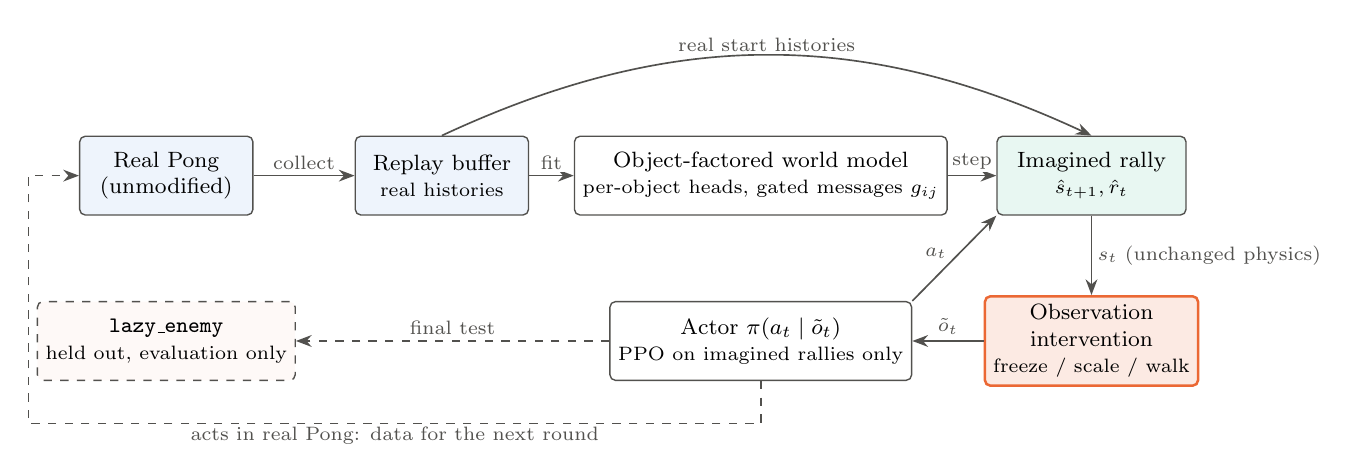
\begin{tikzpicture}[
    box/.style={draw=cink, rounded corners=2pt, align=center, font=\footnotesize, inner sep=3pt,
                fill=white, line width=0.5pt, minimum height=10mm},
    real/.style={box, fill=cblue!8},
    imag/.style={box, fill=caqua!10},
    ours/.style={box, fill=corange!14, draw=corange, line width=0.9pt},
    arr/.style={-{Stealth[length=2mm]}, cink, line width=0.6pt},
    lab/.style={font=\scriptsize, text=cink, fill=white, inner sep=1pt}
  ]
  % row 1: real data -> world model -> imagination
  \node[real, minimum width=22mm] (env) at (0,0) {Real Pong\\(unmodified)};
  \node[real, minimum width=22mm] (buf) at (3.5,0) {Replay buffer\\{\scriptsize real histories}};
  \node[box,  minimum width=33mm] (wm)  at (7.55,0) {Object-factored world model\\{\scriptsize per-object heads, gated messages $g_{ij}$}};
  \node[imag, minimum width=24mm] (imag) at (11.75,0) {Imagined rally\\{\scriptsize $\hat s_{t+1},\hat r_t$}};
  % row 2: intervention -> actor -> evaluation
  \node[ours, minimum width=24mm] (int) at (11.75,-2.1) {Observation\\intervention\\{\scriptsize freeze / scale / walk}};
  \node[box,  minimum width=33mm] (actor) at (7.55,-2.1) {Actor $\pi(a_t\mid\tilde o_t)$\\{\scriptsize PPO on imagined rallies only}};
  \node[box, dashed, fill=corange!4, minimum width=22mm] (lazy) at (0,-2.1) {\lazy{}\\{\scriptsize held out, evaluation only}};
  % arrows
  \draw[arr] (env) -- node[lab, above=1pt]{collect} (buf);
  \draw[arr] (buf) -- node[lab, above=1pt]{fit} (wm);
  \draw[arr] (wm) -- node[lab, above=1pt]{step} (imag);
  \draw[arr] (buf.north) to[out=25, in=155] node[lab, above]{real start histories} (imag.north);
  \draw[arr] (imag) -- node[lab, right=1pt]{$s_t$ (unchanged physics)} (int);
  \draw[arr] (int) -- node[lab, above=1pt]{$\tilde o_t$} (actor);
  \draw[arr] (actor.north east) -- node[lab, above left=0pt and 0pt, pos=0.45]{$a_t$} (imag.south west);
  \draw[arr, dashed] (actor.south) -- (7.55,-3.15) -- node[lab, below]{acts in real Pong: data for the next round} (-1.75,-3.15) -- (-1.75,0) -- (env.west);
  \draw[arr, dashed] (actor.west) -- node[lab, above=1pt]{final test} (lazy.east);
\end{tikzpicture}}
\caption{\textbf{Overview.} Real interaction with unmodified Pong only fills a replay buffer. An
object-factored world model is fitted on it, and the actor is trained with PPO purely on imagined
rallies that start from real histories. Our change (orange) is applied between the imagined state and
the actor: in most rallies the enemy's position \emph{as seen by the actor} is intervened on, while
the imagined dynamics, ball and reward are not. \lazy{} is used only to evaluate the finished actor.}
\label{fig:overview}
\end{figure}

\subsection{Object-factored world model}
\label{sec:wm}

The world model $f_\theta$ maps a history of $K=16$ object states and the action to the next object
states and the reward. Each object $i\in\{\text{player},\text{enemy},\text{ball}\}$ has its own
encoder $e_i = \mathrm{MLP}_i(\text{positions and velocities of } i \text{ over } K \text{ frames})$,
and the action is embedded as a fourth token $e_a$. Object $i$ receives a message from every other
token $j$, scaled by a gate that is recomputed at every step:
\begin{equation}
  m_i = \sum_{j\neq i} g_{ij}\,\mathrm{LN}\big(\mathrm{MLP}^{\text{msg}}_i([e_i, e_j])\big),\qquad
  g_{ij} = \sigma\big(\mathrm{MLP}^{\text{gate}}_i([e_i,e_j])\big)\in[0,1].
  \label{eq:gates}
\end{equation}
A per-object head predicts the displacement $\Delta\hat s_i = \mathrm{MLP}^{\text{dec}}_i([e_i, m_i])$,
and the ball's head also predicts the reward $\hat r\in\{-1,0,+1\}$, since points are events of the
ball. The gates are the model's dependency graph and are regularised with an $L_1$ penalty. We train
with an 8-step open-loop loss in which predictions are fed back as inputs:
$\mathcal{L}=\sum_{k=1}^{8}\big[\sum_i\|\Delta\hat s_{i,t+k}-\Delta s_{i,t+k}\|^2 + \mathrm{CE}(\hat r_{t+k}, r_{t+k}) + \lambda \sum_{i\neq j} g_{ij,t+k}\big]$.
The model learns sensible, time-varying dependencies (Figure~\ref{fig:gates}): the player listens
to the action, and the ball listens to the player and the action only around the player's hits.

\subsection{Actor training in imagination}
\label{sec:ppo}

We treat the world model as a batched JAX environment~\cite{jaxatari}. An imagined episode starts
from a real 16-frame history sampled from the replay buffer and lasts one \emph{rally}: it ends when
the reward head predicts a point, or after 256 steps with value bootstrapping. Ball and enemy
positions are rounded to integers, as in the game. The actor-critic (two $2{\times}256$ MLPs) sees the
last four frames of object positions and their differences, and is trained with PPO~\cite{schulman2017ppo}
and GAE~\cite{schulman2016gae} on 2048 imagined environments. Training proceeds in 5 Dreamer-style
rounds~\cite{hafner2020dreamer}. Each round collects 512k real steps of \emph{unmodified} Pong (round 0
with a random policy, later rounds with the current actor and 10\% random actions), refits the world
model on all data, and runs 400 PPO updates (105M imagined steps) in imagination. The actor never
sees a real transition.

\subsection{Observation interventions}
\label{sec:obsint}

The actor's input is computed from the imagined state $s_t$ with one change: the enemy's height is
replaced by an \emph{observed} enemy track $\tilde y^{e}_t$. At the start of each imagined rally we
sample a mode $c$: \emph{none} with probability $p_{\text{none}}$ (then $\tilde y^{e}=y^{e}$), otherwise
one of three generic interventions on the observed enemy's motion. Writing
$\Delta_t = y^{e}_{t+1}-y^{e}_t$ for the imagined enemy's displacement,
\begin{equation}
  \tilde y^{e}_{t+1} = \mathrm{clip}\big(\tilde y^{e}_t + \tilde\Delta_t\big),\qquad
  \tilde\Delta_t = \begin{cases}
     (1-z_t)\,\Delta_t & \text{freeze; } z_t\in\{0,1\}\text{ flips w.p. } 0.1,\\
     \mathrm{round}(\kappa\,\Delta_t) & \text{scale; } \kappa\sim\mathcal{U}[0,1.5],\\
     \delta_t\sim\mathcal{U}\{-8,-4,0,4,8\} & \text{random walk.}
  \end{cases}
  \label{eq:obsint}
\end{equation}
The switch $z_t$ flips independently at every step, $\kappa$ is drawn once per rally, and the
non-\emph{none} modes are drawn in ratio $2{:}1{:}1$. Crucially, the world model, the ball, the
reward and the \emph{true} enemy are never changed, so every imagined rally is a consistent game of
Pong under the learned dynamics. The actor experiences games in which its view of the enemy is
unreliable, and is rewarded for winning them. We use $p_{\text{none}}=0.1$.

\paragraph{Design choice.} Intervening on the enemy object encodes the assumption that the opponent is
the part of the environment whose behaviour may change. We intervene on the object that the agent
neither controls nor has to hit, and not on the ball, since without the ball the game cannot be
played. The interventions are generic perturbations of one object's motion. They are not the \lazy{}
rule, which conditions the enemy's motion on the ball's direction.

\begin{algorithm}[t]
\caption{Imagination training with observation interventions (one run)}
\label{alg:method}
\begin{algorithmic}[1]
\small
\State $\mathcal{D}\gets\emptyset$; initialise world model $f_\theta$, actor-critic $(\pi_\phi, V_\phi)$
\For{round $=0,\dots,4$}
  \State collect 512k steps of \emph{unmodified} Pong with a random policy (round 0) or $\pi_\phi$ (+10\% random), add to $\mathcal{D}$
  \State fit $f_\theta$ on $\mathcal{D}$ with the 8-step open-loop loss (Section~\ref{sec:wm})
  \For{400 PPO updates}
    \For{each of 2048 imagined envs, 128 steps}
      \If{new rally} sample a real 16-frame history from $\mathcal{D}$ and a mode $c$ (Eq.~\ref{eq:obsint}); $\tilde y^{e}\gets y^{e}$ \EndIf
      \State $\tilde o_t\gets$ actor input from $s_{t-3:t}$ with the enemy's height replaced by $\tilde y^{e}_{t-3:t}$
      \State $a_t\sim\pi_\phi(\cdot\mid\tilde o_t)$;\quad $(\hat s_{t+1},\hat r_t)\gets f_\theta(s_{t-15:t},a_t)$ \Comment{dynamics never intervened}
      \State update $\tilde y^{e}_{t+1}$ from the imagined enemy's displacement and mode $c$ (Eq.~\ref{eq:obsint})
      \State end the rally if $\hat r_t\neq 0$ or after 256 steps (bootstrap with $V_\phi$)
    \EndFor
    \State PPO update of $(\pi_\phi, V_\phi)$ on the imagined batch
  \EndFor
  \State save candidate checkpoints (greedy and sampled actions)
\EndFor
\State select a candidate with the unmodified-Pong rule (Section~\ref{sec:selection}); evaluate once on \lazy{}
\end{algorithmic}
\end{algorithm}

\subsection{Selection without the test modification}
\label{sec:selection}

Each run yields 10 candidates (5 rounds $\times$ greedy/sampled actions). We choose the one with the
highest mean of two final scores, both measured on unmodified Pong (32 games each): normal play, and
play in which the agent's view of the enemy is frozen at a random height for the whole game, a generic
sensor-failure check. The rule was fixed before the runs reported for our main configuration, and we
apply it to every method.

% ------------------------------------------------------------------------------------------
\section{Experiments}
\label{sec:results}

\paragraph{Methods compared.} \textbf{WM + MLP actor} (Exp.~1): the world model of
Section~\ref{sec:wm} and PPO in imagination, without interventions. \textbf{Dynamics interventions}
(Exp.~2): the same pipeline with $L_0$ gates~\cite{louizos2018l0}, where the interventions of
Eq.~\eqref{eq:obsint} are applied to the \emph{world model's} enemy prediction (with probability 0.75
per rally), so the imagined ball reacts to the intervened enemy. \textbf{Gated actor} (Exp.~3): an
actor whose ball and enemy inputs pass through per-step hard-concrete gates with an expected-$L_0$
penalty, so it can learn to ignore the enemy. \textbf{Observation interventions} (ours) with
$p_{\text{none}}=0.4$ and $0.1$. All methods share the data pipeline, PPO settings and selection rule,
and all except Exp.~2 share the world model. Each run takes about 40 minutes on one A100 GPU. We report the mean and standard
deviation over seeds, and all 32 games per seed.

\begin{figure}[t]
  \centering
  \figinc{figures/main_results.pdf}
  \caption{\textbf{Final score on unmodified Pong and under the held-out \lazy{} modification.} Bars:
  mean over seeds; dots: individual seeds (32 games each); dashed: success threshold $+10$. All
  methods win unmodified Pong clearly. Only observation interventions stay robust under \lazy{}.}
  \label{fig:main}
\end{figure}

\begin{table}[t]
  \caption{\textbf{Main results.} Final score (agent $-$ enemy points, mean $\pm$ std over seeds, 32
  games per seed). ``Frozen view'' is the selection proxy on unmodified Pong. \lazy{} is the held-out
  test.}
  \label{tab:main}
  \centering
  \small
  \setlength{\tabcolsep}{4pt}
  \begin{tabular}{lccccc}
    \toprule
    Method & seeds & Pong & Pong, frozen view & \lazy{} & won \\
    \midrule
    \MainTableRows
    \bottomrule
  \end{tabular}
\end{table}

\subsection{Main result}

Figure~\ref{fig:main} and Table~\ref{tab:main} summarise the results. Imagination training works:
every method wins unmodified Pong clearly, although its actor never experienced a real transition. The
baseline's strength is brittle. Under \lazy{} it loses (\BaseLazy{}\,$\pm$\,\BaseLazyStd{}), and the
gated actor fares no better (\GatedLazy{}): its enemy gate stays open, because in unmodified Pong the
enemy is genuinely informative. Dynamics interventions improve the \lazy{} score to \DynLazy{} but
fall far short of the goal. Observation interventions with $p_{\text{none}}=0.1$ reach
\OursLazy{}\,$\pm$\,\OursLazyStd{} (range \OursLazyMin{} to \OursLazyMax{} over seeds; worst single game
\OursWorstGame{}) and win \OursWon\% of all \lazy{} games, while scoring \OursPong{} on unmodified Pong.
Figure~\ref{fig:pergame} shows the distribution over individual games: the baselines lose most
\lazy{} games, while our agents win nearly all of them by large margins. Figure~\ref{fig:traces}
illustrates the failure. In normal Pong, the enemy's height tracks the ball's while the ball
travels towards the player, and the baseline's paddle is drawn towards the enemy's height even when
it no longer says anything about the ball.

\begin{figure}[t]
  \centering
  \figinc{figures/per_game.pdf}
  \caption{\textbf{Final score of every \lazy{} game} (all seeds pooled; bar: median, whisker:
  interquartile range; top: share of games won).}
  \label{fig:pergame}
\end{figure}

\begin{figure}[t]
  \centering
  \figinc{figures/traces_lazy.pdf}
  \caption{\textbf{Behaviour under \lazy{}.} Left: the baseline's first lost point in a \lazy{} game.
  After returning the ball, the \lazy{} enemy (magenta) stays where it hit it. The baseline's paddle
  (aqua) first follows the ball down, then moves back up towards the stale enemy's height and misses
  the ball by a few pixels. All three points it lost in the first 600 steps of this game look alike.
  Right: our agent in a comparable situation (enemy $\geq 40$\,px from the ball when it arrives)
  stays with the ball and returns it.}
  \label{fig:traces}
\end{figure}

\subsection{Why intervening inside the world model fails: leakage}
\label{sec:leakage}

If the world model were object-contained, interventions on its enemy (Exp.~2) would produce valid
counterfactual games. We test containment with a \emph{counterfactual leakage} test: on real
held-out windows we replace object $j$'s entire history by that of a random other window, and measure
how much object $i$'s one-step prediction changes. For the ball and the enemy, a contained model
should change only near the enemy's paddle. Figure~\ref{fig:leakage} shows three findings.
(a)~Removing the ball's messages from the enemy entirely costs little: the mean one-step error rises
from 0.71 to 0.90\,px, mostly in the bounce zone. (b)~Yet the model uses the enemy when the ball is
far away, and the effect grows with the enemy-ball gap after the swap. Gaps above 40\,px never occur
in real data, where the enemy tracks the ball, and there the ball's prediction moves by more than
20\,px. (c)~Pairwise $L_0$ gates, receiver-driven $L_0$ gates, receiver-driven soft gates with exact
zeros, and receiver-driven straight-through binary gates all keep a far-field leakage of 10--14\,px.
Receiver-driven $L_0$ gates even collapsed to state-independent constants and stopped the ball from
listening to the player. A penalty on the training loss cannot tell ``useful in training'' from
``causally needed'' when two objects are this correlated. Consequently, intervening on the enemy
inside the model also moves the imagined ball, and the actor learns that the enemy matters for the
ball's trajectory. Observation interventions avoid the problem: they never feed an unseen enemy into
the world model.

\begin{figure}[t]
  \centering
  \figinc{figures/leakage.pdf}
  \caption{\textbf{World-model leakage from enemy to ball.} (a) Ablation: the ball's one-step error
  with and without messages from the enemy, by ball position. (b) Change of the ball's prediction when
  the enemy's history is swapped, by the resulting enemy-ball gap (ball moving, far from the enemy).
  The shaded band covers the gaps that occur in real data. (c) Far-field and near-field leakage for
  gating variants.}
  \label{fig:leakage}
\end{figure}

\subsection{The world model is not robust, but the actor is}

\begin{figure}[t]
  \centering
  \begin{minipage}[t]{0.49\linewidth}
    \figinc{figures/training.pdf}
    \caption{\textbf{Real Pong final score after each round} (greedy actor; thin: seeds, thick: mean).}
    \label{fig:training}
  \end{minipage}\hfill
  \begin{minipage}[t]{0.49\linewidth}
    \figinc{figures/frozen_proxy.pdf}
    \caption{\textbf{Selection proxy vs.\ held-out score.} Each point is one selected run.}
    \label{fig:proxy}
  \end{minipage}
\end{figure}

Figure~\ref{fig:wmerror} shows the open-loop error of our agent's world model on real trajectories.
Under \lazy{}, the enemy's prediction is wrong, as expected for a changed mechanism. Because of the
leakage above, the ball's prediction degrades too (1.0\,px to 4.2\,px after one step). The world model
is therefore \emph{not} robust. The actor is robust anyway, because it was trained to succeed under
unreliable enemy information while the imagined ball stayed consistent. The gates of the world model
(Figure~\ref{fig:gates}) remain interpretable. The ball listens to the player and the action only
around the player's hits, and the enemy listens to the ball. The ball also listens to the enemy
whenever the ball approaches it, which is the far-field dependence measured above.

\begin{figure}[t]
  \centering
  \figinc{figures/wm_error.pdf}
  \caption{\textbf{Open-loop world-model error} (our agent's world model, 4096 windows of its own
  real trajectories) on unmodified Pong and under \lazy{}.}
  \label{fig:wmerror}
\end{figure}

\begin{figure}[t]
  \centering
  \figinc{figures/gates.pdf}
  \caption{\textbf{Interaction gates of the world model along a real Pong trajectory.} Top: ball $x$
  with the paddles' $x$ ranges. Middle: gates of the ball. Bottom: gates of the enemy.}
  \label{fig:gates}
\end{figure}

\subsection{Ablations and analysis}

\paragraph{Fraction of intervened rallies.} With $p_{\text{none}}=0.4$ (interventions in 60\% of
rallies) the result depends on the seed. One seed is robust and the other still loses many \lazy{}
games (\OursSixtyLazy{}\,$\pm$\,\OursSixtyLazyStd{}; Table~\ref{tab:main}). The agent can learn to
trust the enemy when its track ``looks normal''. With interventions in 90\% of rallies all seeds are
robust. More interventions did not cost performance on the unmodified game (Figure~\ref{fig:training}).

\paragraph{The selection proxy.} Figure~\ref{fig:proxy} plots the frozen-view score, measured on the
unmodified game, against the held-out \lazy{} score for every selected run. Agents that collapse when
their view of the enemy is frozen also fail under \lazy{}. The clearest case is the baseline (seed 0):
$+19.0$ on Pong, $-10.6$ with a frozen enemy view, and $-8.4$ under \lazy{}. The proxy is
therefore a useful, test-free warning sign. It is not sufficient, however. One run with 60\%
interventions is unaffected by the frozen view ($+18.5$) but reaches only $+3.1$ under \lazy{}: an
enemy that is frozen for the whole game is a different perturbation from one that is sometimes
still and sometimes moving. In all our runs the proxy selected the same checkpoint as the plain Pong
score, so it did not change any reported result.

\paragraph{Imagined vs.\ real robustness.} In imagination, our actor wins the same share of points
with and without an intervened enemy view (\eg 0.94 vs.\ 0.94 in the last round of seed 0), so its
imagined success does not depend on the enemy. Appendix~\ref{app:imagination} shows imagined rollouts
next to reality.

% ------------------------------------------------------------------------------------------
\section{Discussion and limitations}
\label{sec:discussion}

\paragraph{What the result does and does not show.} Our agents are robust to a changed opponent
mechanism because they were trained not to rely on the opponent's position, and imagination made
that training cheap and physically consistent. The world model itself is not object-contained, and
our leakage analysis suggests that sparsity regularisation alone will not make it so when objects
are strongly correlated in the training data. Interventional data, or stronger priors such as
locality, would be needed.

\paragraph{Assumptions and possible leakage of test knowledge.} Choosing the enemy as the object to
intervene on encodes a prior about which part of the environment may change. Our interventions are
generic (freeze, scaled motion, random walk), but the \emph{freeze} family resembles the stale enemy of
\lazy{} more than, \eg, an enemy that moves faster than the ball. The fraction $p_{\text{none}}=0.1$
was chosen after observing the $p_{\text{none}}=0.4$ runs on \lazy{}, so the main configuration is not
a fully blind test of that hyperparameter. For this reason we report both settings. The selection rule
was fixed before the main runs, and every selected checkpoint was evaluated on \lazy{} once.

\paragraph{Scope.} We study one game, one modification and a small number of seeds, with
ground-truth object states from JAXAtari rather than learned object representations. Whether
observation interventions scale to games with many interacting objects, where the object to intervene
on is less obvious, remains open. A natural extension is to intervene on every non-controlled object
in turn and to use the frozen-view proxy per object to find the objects the agent should not rely on.

% ------------------------------------------------------------------------------------------
\section{Conclusion}

An imagination-trained agent is only as robust as the correlations it was allowed to exploit. In
object-centric Pong, the opponent's position is such a correlation, and it is absorbed both by the
world model and by the actor. Making the world model object-contained through sparsity did not remove
it. Intervening on the model's dynamics was harmful, because the leaking model turns those
interventions into false physics. Intervening on what the actor \emph{sees}, while keeping the imagined
physics intact, produced agents that win the held-out \lazy{} game with a final score of
\OursLazy{}\,$\pm$\,\OursLazyStd{} across \OursSeeds{} seeds, without ever training, tuning or selecting
on it.

\begin{ack}
Experiments, code and a first draft of this paper were produced with the help of an AI coding
assistant (Claude, Anthropic) working under the author's direction. All numbers are generated from the
released evaluation files.
\end{ack}

\bibliographystyle{abbrvnat}
\bibliography{references}

% ------------------------------------------------------------------------------------------
\newpage
\appendix

\section{Hyperparameters}
\label{app:hparams}

\begin{table}[h]
  \caption{Hyperparameters (shared by all methods unless noted).}
  \centering
  \small
  \begin{tabular}{p{0.39\linewidth}p{0.55\linewidth}}
    \toprule
    \multicolumn{2}{l}{\emph{Environment}}\\
    JAXAtari Pong, object-centric wrapper & frame skip 4, frame stack 4, sticky actions 0.25, $\leq$30 no-op resets\\
    State used & $(x, y)$ of player, enemy, ball per frame \\
    \midrule
    \multicolumn{2}{l}{\emph{Data collection (per round)}}\\
    Rounds & 5 \\
    Real steps per round & $256$ envs $\times$ 2000 steps $= 512$k (round 0: random policy) \\
    Collection policy (rounds $\geq 1$) & current actor, 10\% random actions \\
    \midrule
    \multicolumn{2}{l}{\emph{World model}}\\
    History $K$ / open-loop training horizon $H$ & 16 / 8 \\
    Width & 128 (encoders, messages, decoders: 2-layer MLPs, GELU) \\
    Gate penalty $\lambda$ & 0.01 ($L_1$ on sigmoid gates) \\
    Optimiser & AdamW, lr $3\cdot10^{-4}$, weight decay $10^{-4}$, grad-norm clip 1.0 \\
    Batch / steps per round & 512 windows / 20k (continues from the previous round) \\
    \midrule
    \multicolumn{2}{l}{\emph{Imagination and PPO}}\\
    Imagined envs / rollout length & 2048 / 128 steps \\
    Episode & one rally (ends at a predicted point) or 256 steps (value bootstrap) \\
    PPO updates per round & 400 ($\approx$105M imagined steps) \\
    Epochs / minibatches / clip & 4 / 8 / 0.2 \\
    lr / $\gamma$ / GAE $\lambda$ & $3\cdot10^{-4}$ / 0.99 / 0.95 \\
    Entropy / value coefficients & 0.01 / 0.5 \\
    Actor, critic & separate $2\times256$ ReLU MLPs; input: 4 frames of positions + differences (42 dims) \\
    \midrule
    \multicolumn{2}{l}{\emph{Observation interventions (ours)}}\\
    $p_{\text{none}}$ & 0.1 (ablation: 0.4) \\
    Mode ratio freeze : scale : random walk & 2 : 1 : 1 \\
    Freeze switch prob. / scale range / walk steps & 0.1 per step / $\mathcal{U}[0,1.5]$ / $\{-8,-4,0,4,8\}$ px \\
    \midrule
    \multicolumn{2}{l}{\emph{Selection and evaluation}}\\
    Candidates & 5 rounds $\times$ \{greedy, sampled\} \\
    Selection score & mean of Pong and frozen-view Pong final score (32 games each) \\
    Evaluation & 32 full games per environment, max 10{,}000 agent steps \\
    \bottomrule
  \end{tabular}
\end{table}

\section{Imagination vs.\ reality}
\label{app:imagination}

\begin{figure}[H]
  \centering
  \figinc{figures/imagination.pdf}
  \caption{\textbf{Open-loop imagination} of our agent's world model (dots) against the real
  trajectory (lines), 16 frames of real context followed by 40 imagined steps with the real actions.
  On unmodified Pong the imagined ball and paddles stay close to reality for the whole window. Under
  \lazy{} the imagined enemy keeps tracking the ball as it did in training while the real enemy stays
  still, and the imagined ball diverges from the real one after roughly ten steps. The world model does
  not transfer to the changed game.}
  \label{fig:imagination}
\end{figure}

\section{Further negative results}
\label{app:negative}

\paragraph{Gated actor.} Penalising the actor's attention to objects (hard-concrete gates with an
expected-$L_0$ penalty) either closed \emph{all} gates before the actor had learned to play, when the
penalty was active from the start (the actor lost $0.3{:}21$), or none of them, when the penalty was
applied after a warm-up. A reward-driven penalty cannot remove information that is useful in training.

\paragraph{Receiver-driven gates.} Deciding the gate $g_{ij}$ from the receiver's state only,
$g_{ij}=\sigma(f_i(e_i))_j$, guarantees that a closed gate makes $i$ invariant to $j$. With
hard-concrete gates, the gates collapsed to constants. With soft gates (zeroed below 0.1 at use time)
or straight-through binary gates, they stayed open for ball $\leftarrow$ enemy in free flight
(Figure~\ref{fig:leakage}c). The ball's error was similar in all variants, so the open gate buys very
little accuracy. It nonetheless survives the penalty, which suggests that the optimisation finds the
enemy a convenient, low-noise source of the ball's height.

\paragraph{Compute.} All experiments ran on two A100 GPUs. One training run takes about 40 minutes, and
selection plus evaluation take about 30 minutes per run.

% ------------------------------------------------------------------------------------------
\newpage
\section*{NeurIPS Paper Checklist}

\begin{enumerate}[leftmargin=*]
\item {\bf Claims.} Do the main claims made in the abstract and introduction accurately reflect the
paper's contributions and scope? \answerYes{} The claims are restricted to object-centric Pong and the
\lazy{} modification (Sections~\ref{sec:setting}, \ref{sec:results}, \ref{sec:discussion}).
\item {\bf Limitations.} \answerYes{} Section~\ref{sec:discussion}.
\item {\bf Theory assumptions and proofs.} \answerNA{} No theoretical results.
\item {\bf Experimental result reproducibility.} \answerYes{} Section~\ref{sec:method},
Appendix~\ref{app:hparams}; the code, commands and evaluation files are released with the paper.
\item {\bf Open access to data and code.} \answerYes{} All data is generated by the released code from
the open-source JAXAtari environment.
\item {\bf Experimental setting/details.} \answerYes{} Appendix~\ref{app:hparams}.
\item {\bf Experiment statistical significance.} \answerYes{} Mean and standard deviation over seeds,
per-seed points and per-game distributions (Figures~\ref{fig:main}, \ref{fig:pergame}). The number of
seeds is small, and some baselines have a single seed.
\item {\bf Experiments compute resources.} \answerYes{} Appendix~\ref{app:negative} (Compute).
\item {\bf Code of ethics.} \answerYes{}
\item {\bf Broader impacts.} \answerNA{} Foundational research on robustness in a video game, with no
direct societal impact beyond general progress in RL robustness.
\item {\bf Safeguards.} \answerNA{}
\item {\bf Licenses for existing assets.} \answerYes{} JAXAtari~\cite{jaxatari} is cited; its license
applies to the environment.
\item {\bf New assets.} \answerNA{}
\item {\bf Crowdsourcing and research with human subjects.} \answerNA{}
\item {\bf IRB approvals.} \answerNA{}
\item {\bf Declaration of LLM usage.} \answerYes{} An AI coding assistant was used to implement the
experiments and draft the paper (Acknowledgements).
\end{enumerate}

\end{document}
